\documentclass{beamer} 
\usepackage{multicol}
\usepackage{url}
\usepackage{fancyvrb}
\usepackage{color}

\title{What every programmer should know about merging branches in Mercurial} 
\author{Sergey Kishchenko} 
\date{\today} 
\usetheme{CambridgeUS}
\usecolortheme{seagull}
\institute{DoctorMobile}

\begin{document}

\frame{\titlepage}

\begin{frame} 
\frametitle{Branches}
\begin{multicols}{2}
\center{Two different branches}
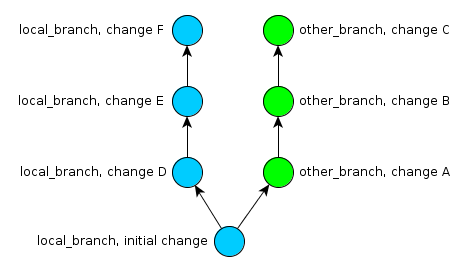
\includegraphics[width=0.4\textwidth]{img/two_branches}
\columnbreak
\center{Two different defaults}
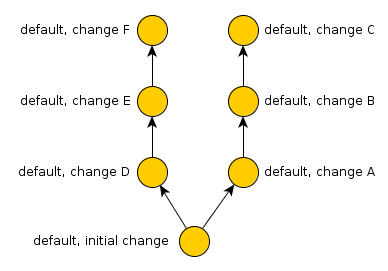
\includegraphics[width=0.4\textwidth]{img/two_default_branches}
\end{multicols}
\begin{itemize}
\item \textbf{NOTE}: Different repos cloned from one source are not actually different, they are more like one repo. You can transfer changes between them with push and pull
\item \textbf{IMPORTANT}: Branches in Mercurial are permanent!
\end{itemize}
\end{frame}

\begin{frame}[fragile]
\frametitle{Pull}
\begin{exampleblock}{First step in merge process: pulling remote changes}
\begin{verbatim}
> hg pull -b REMOTE_BRANCH REMOTE_REPO
\end{verbatim}
\end{exampleblock}
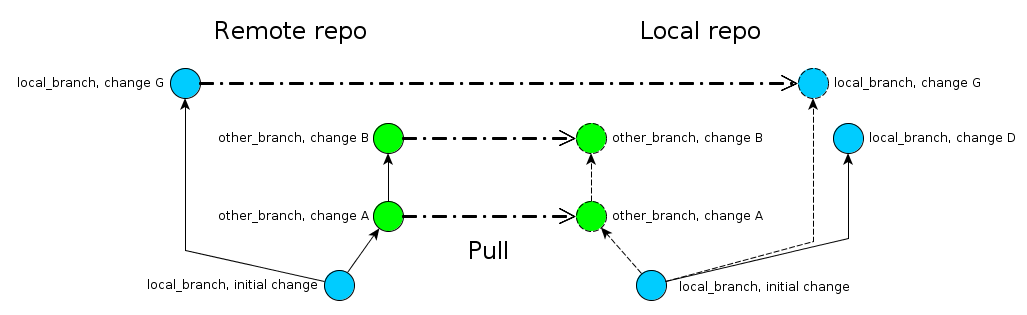
\includegraphics[width=\textwidth]{img/pull_branches}
\begin{itemize}
\item Pulling changes results in pulling all its ancestors
\item Pulling changes may result in creating new heads in branches 
\end{itemize}
\end{frame}

\begin{frame} 
\frametitle{Solutions}
\begin{itemize}
\item Use branches alternatives (bookmarks, lbranches)
\item Use "early-fix" branches 
\item Use graft
\end{itemize}
\end{frame}

\begin{frame} 
\frametitle{Branches alternatives}
TODO
\end{frame}

\begin{frame}
\frametitle{"Early-fix" branches}
TODO
\end{frame}

\begin{frame}
\frametitle{Graft}
TODO
\end{frame}

\begin{frame}[fragile]
\frametitle{Merge}
\begin{exampleblock}{Naïve approach}
\begin{verbatim}
> hg co local_branch
> hg merge remote_branch
or usually (while in default)
> hg pull 
> hg merge 
\end{verbatim}
\end{exampleblock}
\begin{multicols}{2}
\center{Merging different branches}
Image with merged branches
% \includegraphics[width=0.4\textwidth]{img/delorean-blueprint}
\columnbreak
\center{Merging default}
Image with merged defaults
% \includegraphics[width=0.4\textwidth]{img/delorean}
\end{multicols}
\begin{center}
Isn't always so good :( 
% \includegraphics[width=0.45\textwidth]{img/chubaka}
\end{center}
\end{frame}

\begin{frame}
\frametitle{Probable issues}
\begin{itemize}
\item Too much conflicts
\item Hard to understand the conflict
\item Code was refactored
\item Non-source files conflicts
\end{itemize}
\end{frame}

\begin{frame}
\frametitle{Too much conflicts}
TODO: Why occurs? How to prevent? How to deal with? 
\end{frame}

\begin{frame}
\frametitle{Hard to understand the conflict}
TODO: Why occurs? How to prevent? How to deal with? 
\end{frame}

\begin{frame}
\frametitle{Code was refactored}
TODO: Why occurs? How to prevent? How to deal with? 
\end{frame}

\begin{frame}
\frametitle{Non-source files conflicts}
TODO: Why occurs? How to prevent? How to deal with? 
\end{frame}


\begin{frame}
\frametitle{One more time: good things}
\begin{itemize}
\item Specifying branch for pulling
\item Using graft
\item Using good graphical tool for merging
\item Using 3-way merge
\item Using "early-fix" branches
\item Getting knowledge from others when merging theirs code
\item Providing help to those who merge your code
\item Avoiding unnecessary refactoring when
\end{itemize}
\end{frame}

\begin{frame}
\frametitle{One more time: bad things}
\begin{itemize}
\item Manual merges
\item Applying patches manually
\item Being a coward and selecting one side
\item Trusting automatic merge tools completely
\end{itemize}
\end{frame}

\begin{frame}
\frametitle{One more time: things to avoid}
\begin{itemize}
\item Doing a refactoring that can't be merged into all branches immediately
\item Modifying non-source file without merging it into all branches immediately
\item Modifying a component that somebody is working on without notifying him 
\end{itemize}
\end{frame}


\begin{frame}
\frametitle{Thank you! Questions?}
\begin{center}
% \includegraphics[width=0.45\textwidth]{img/chubaka}
\end{center}
\end{frame}

\end{document}
